
% \section{Verification Test}
\section{\change{Testing}}

We now \change{test} tree T1 on the original simulation results from \citet{Taborda_2014_BSSA}, for different velocity models and components of motion. In this case we no longer aggregate all data from the simulation but now look at individual simulations done with different velocity models, and the three components of motion separately, as it would normally be done during any ground motion simulation validation. The results obtained with the T1 validation algorithm are shown in Fig.~\ref{fig:res-gof-maps}. \change{In an ideal case, we would expect these results to closely resemble those obtained by \citet{Taborda_2014_BSSA}, if grouped only into four categories. Relying only on the two metrics C4 and C8 using T1 is, however, not exactly the same. In addition, a}
% 
% These results are in essence very similar to those obtained by \citet{Taborda_2014_BSSA}, though using the T1 algorithm, we now rely only on the two metrics C4 and C8.
% 
% A relative 
drawback from the T1 algorithm is that because its outcome are GOF validation classes (poor, fair, good, excellent) as opposed to GOF validation scores (with values from 0 to 10), once one obtains the results for the validation process for different components of motion (as shown in the rows of Fig.~\ref{fig:res-gof-maps}), there is no natural way of taking averages as one would do for scores in a numerical scale \change{\citep[i.e., as typically done when using][]{Anderson_2004_Proc}}. Therefore, in order to combine results from the three components into a single validation classification for each station, we define the following rules:

\begin{itemize}
	\setlength\itemsep{0ex}
	\item If the three components share the same validation class, then that class is assigned as the combination result.
	\item If two components share the same validation class, but one differs, then the class shared by the former two is assigned as the combination result, thus favoring the majority.
	\item If all three components have different validation classes, then the final combination result is set as the lower class of the three, penalizing the lack of conclusive results.
\end{itemize}

We call the result of applying these rules a tree T1 combination. Applying them to the validation results shown in Fig.~\ref{fig:res-gof-maps} for the case of the simulation done using the model CVM-S is shown in Fig.~\ref{fig:avg-gof-maps}, which compares the outcome with the result of the average scores obtained using the traditional \citet{Anderson_2004_Proc}-type GOF method. This figure exemplifies the \change{differences or similarities} between the numeric GOF validation-scores scale and the proposed T1 GOF validation classes. 
% At the same time, it highlights the similarities between the outcomes.

\begin{figure*}%[th!]
	\centering
	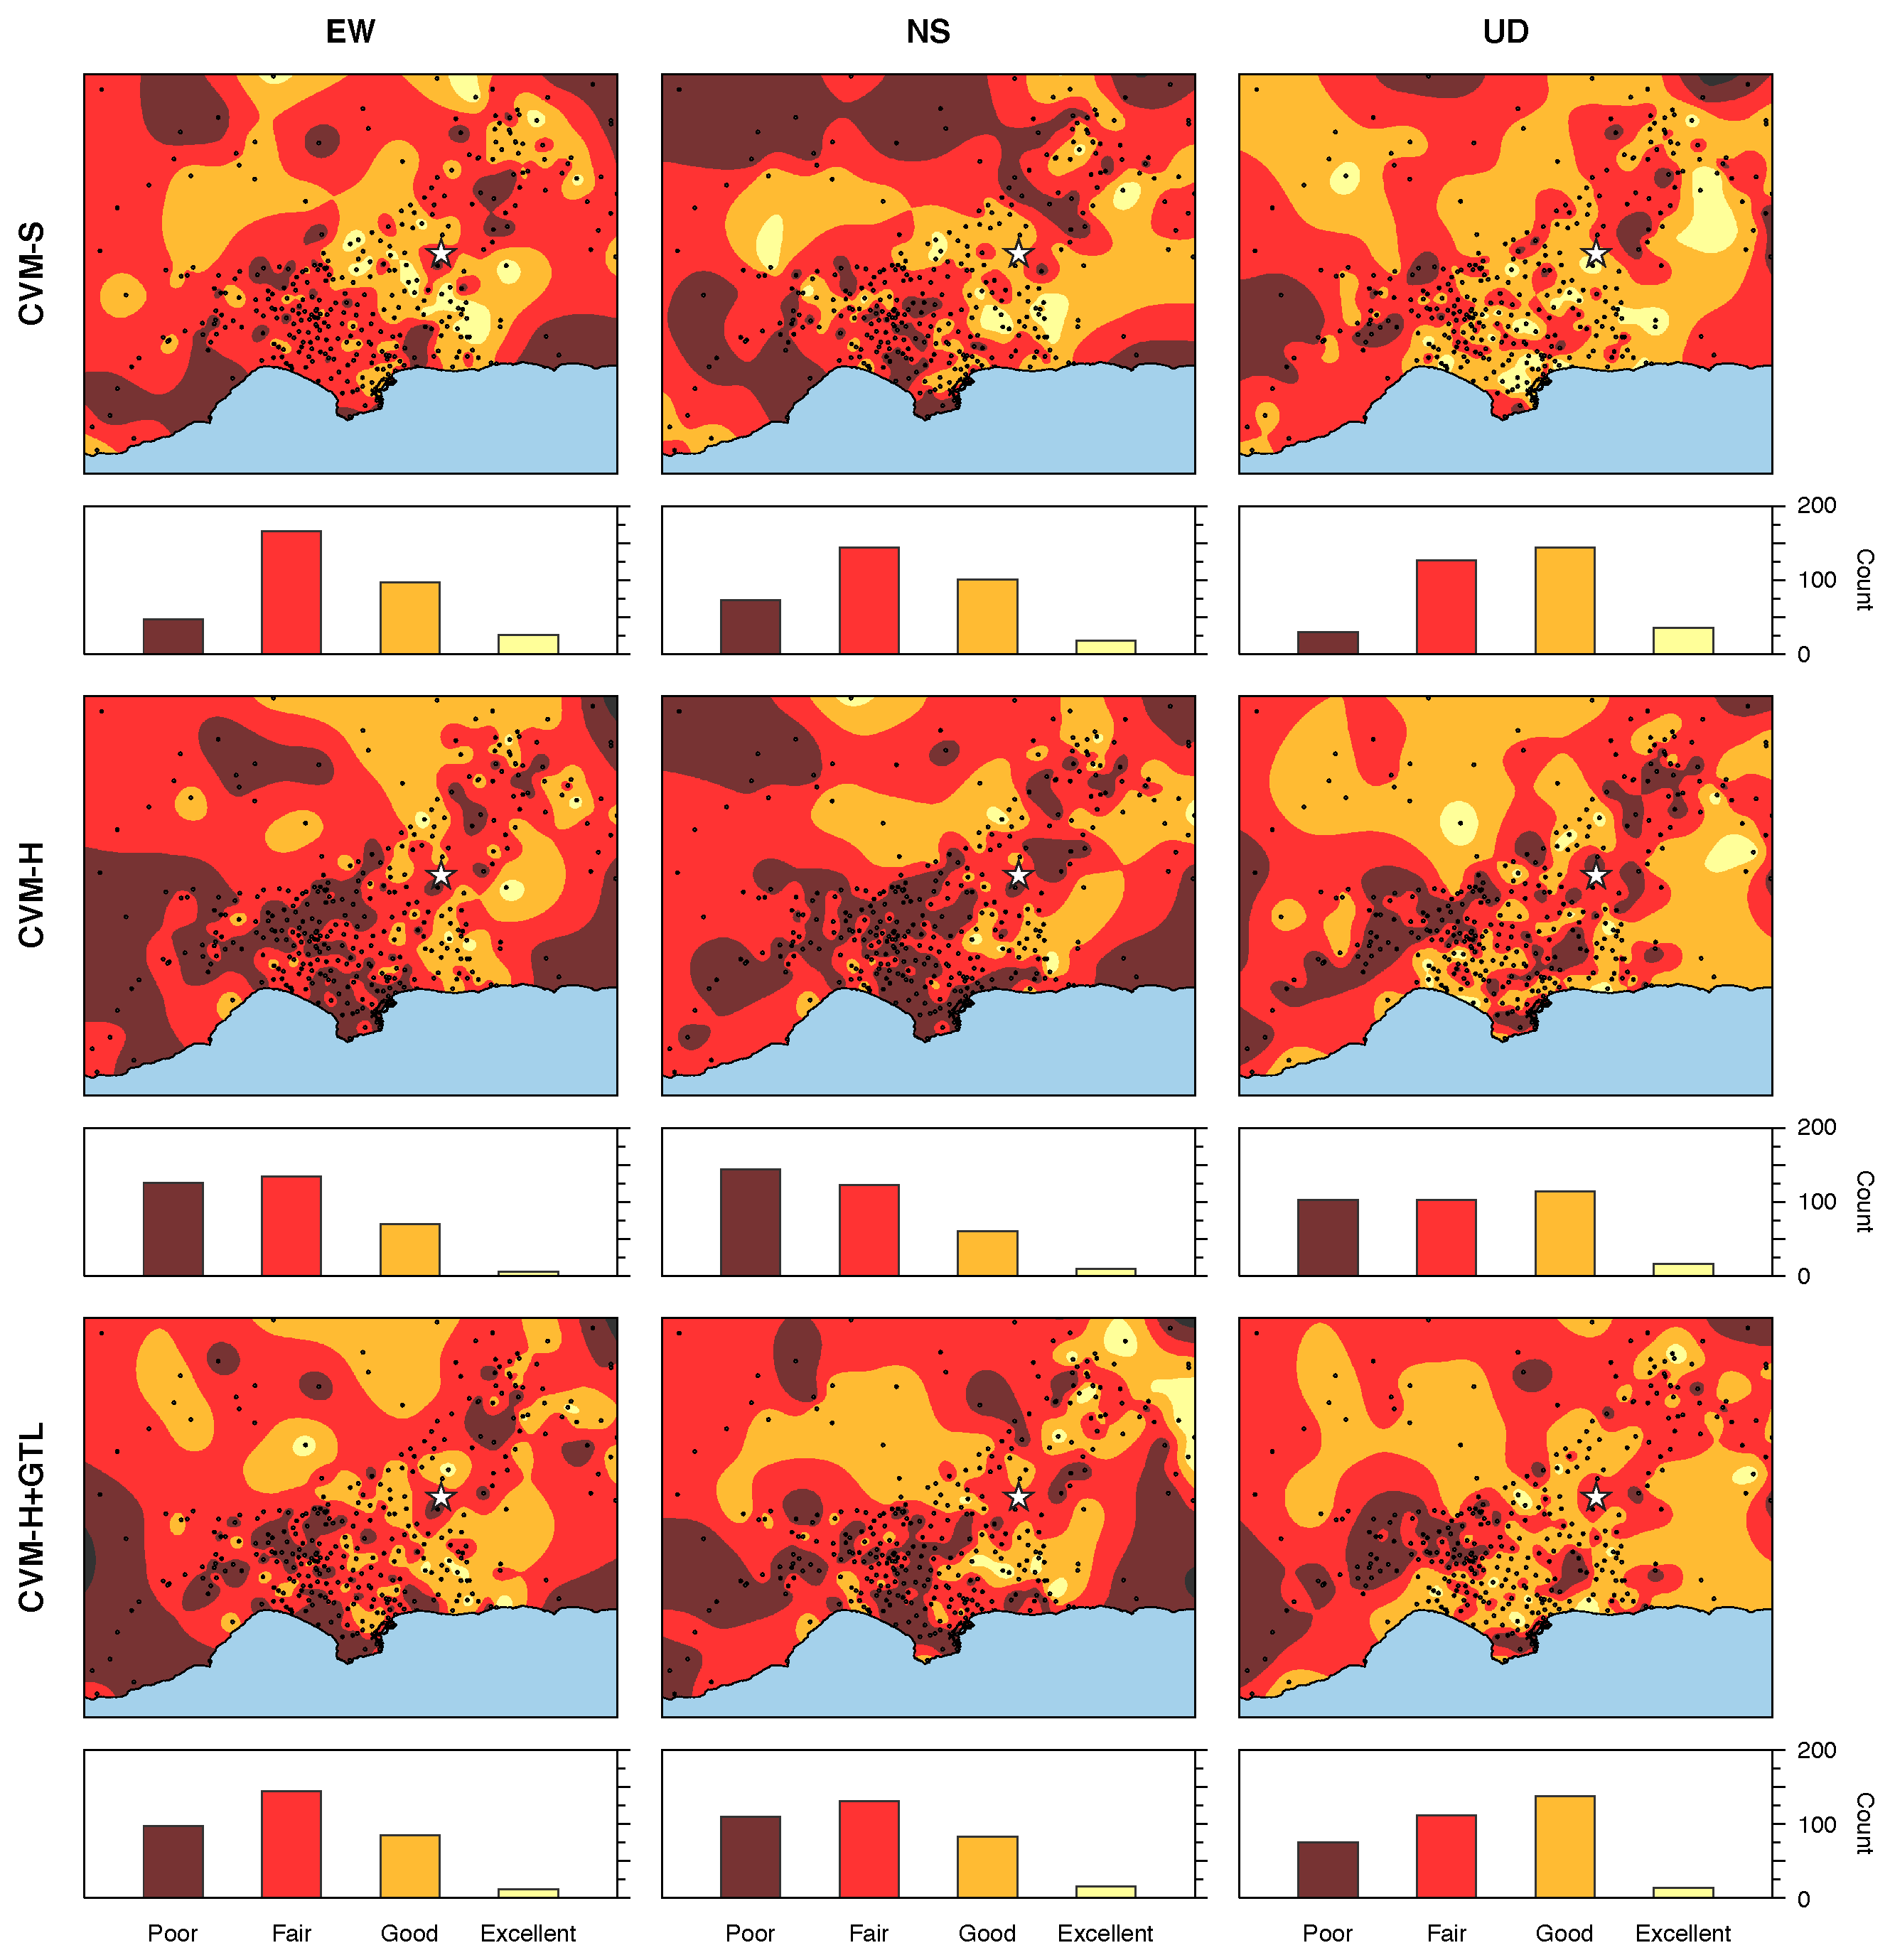
\includegraphics[width=\textwidth]{figures/pdf/figure-10}
	\caption{Results obtained using the validation algorithm of the selected decision tree T1 on the 2008 Chino Hills earthquake simulation results reported by \citet{Taborda_2014_BSSA}. Here, the validation process is carried out separately for each component of motion (EW, NS, UD), for three different simulations corresponding to simulations done using the southern California velocity models: CVM-S, CVM-H, CVM-H+GTL. The contours maps are drawn for illustration purposes only based on the spatial distribution of the GOF validation class assigned to each station. The bottom histograms show the count of stations in each validation class. Stations are indicated with dots, and the epicenter with a Star. The color version of this figure is available only in the electronic edition.}
	\label{fig:res-gof-maps}
\end{figure*}

In our view, the T1 results are simpler to assimilate and equally informative. Looking at both plots in Fig.~\ref{fig:avg-gof-maps} it is possible to argue they lead to \change{similar conclusions in respect to the overall validation of the simulation, and in respect to some particular areas and specific locations. Nonetheless, it must be said that we do not expect to see a 1-to-1 relationship. That is the scope of a future work, whereas here our focus was on identifying the relevance of the different metrics. This is important because the original approach proposed by \citet{Anderson_2004_Proc} favors a uniform weighing of metrics, and the results shown here indicate this may not be the preferred strategy.}

% conclusions and present a similar picture of the validation of the simulation, not only globally but at specific locations, with only minor differences---especially if one is to consider the assumed equivalence between scores and classes (0--4: poor; 4--6: fair; 6--8:good; 8--10: excellent). \myrevision{However, we do not expect to see the same results in both figures. \citet{Taborda_2014_BSSA} results is developed based on assigning uniform weight on all metrics, however, this study research question is addressing the importance of different metrics and implying that assigning uniform weights might not provide accurate results.}

\begin{figure*}[th!]
	\centering
	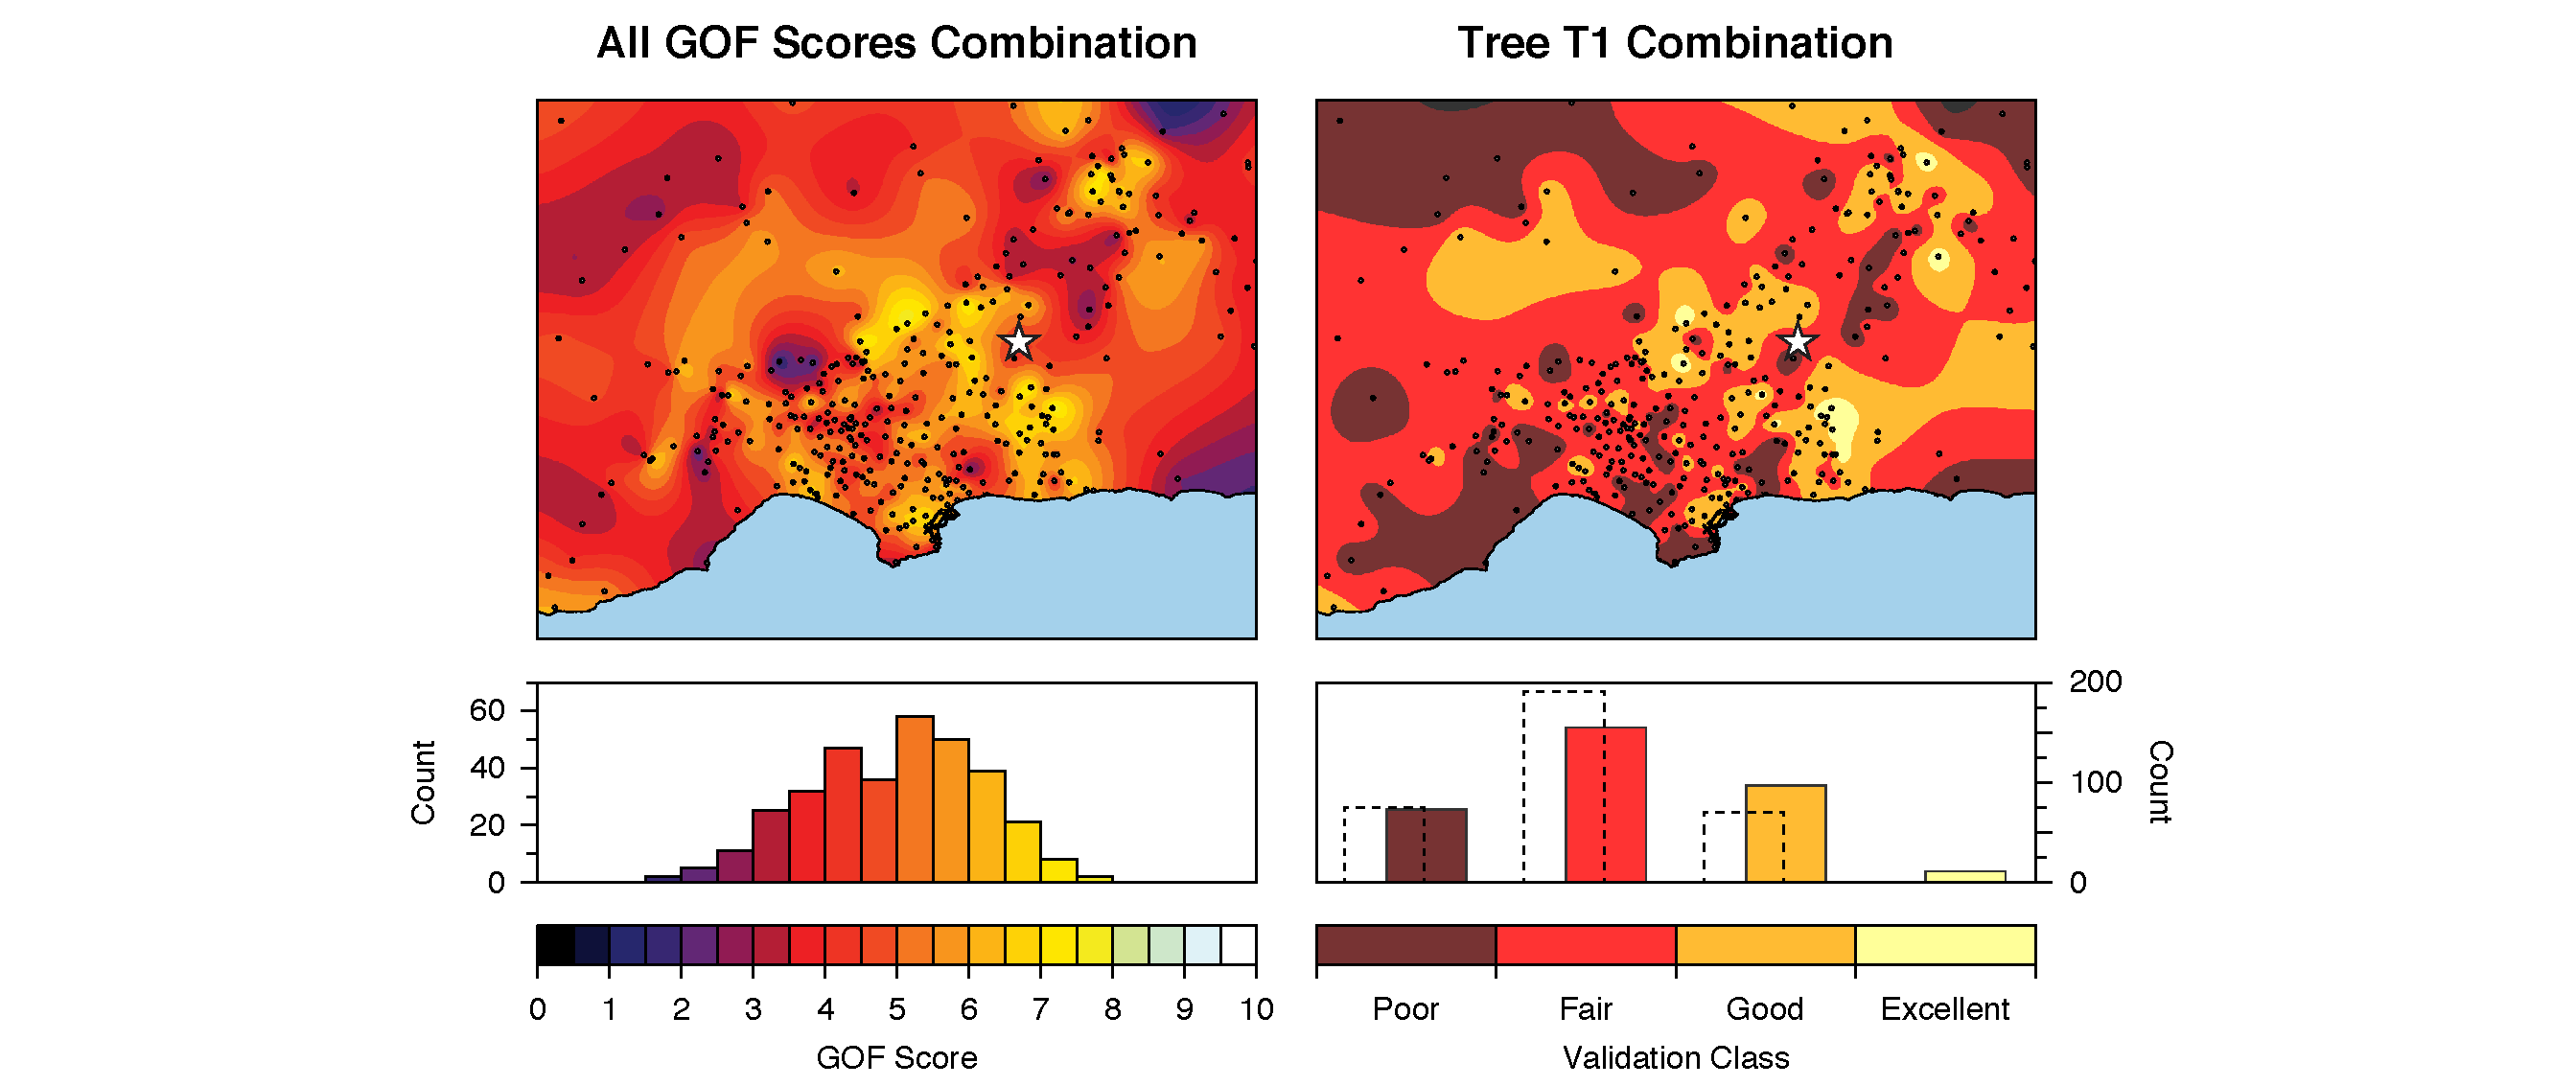
\includegraphics[width=\textwidth]{figures/pdf/figure-11}
	\caption{Comparison of GOF validation scores obtained using an 11-metric \citet{Anderson_2004_Proc}-type GOF scoring (left) and the T1 combination GOF validation classification (right). The top plots show maps with a distribution of the scores or classes outcome at each station. The contours are drawn for illustration purposes only. The bottom plots show histograms with the count of stations for each GOF score interval or validation class.}
	\label{fig:avg-gof-maps}
\end{figure*}

% \myrevision{It is worth mentioning that, in this study, we presented an integration of scientists knowledge and field data using machine learning algorithms to develop an acceptable and robust prediction model. This method can be used in any field where there are some field data as well as expertise knowledge about the data. Validation metrics are note limited to \citeauthor{Anderson_2004_Proc}'s metrics. Therefore, adding more metrics from different field can be used through the proposed method to develop prediction models. }






